\documentclass[a4paper,14pt]{article}
\usepackage{float}
\usepackage{extsizes}
\usepackage{amsmath}
\usepackage{amssymb}
\everymath{\displaystyle}
\usepackage{geometry}
\usepackage{fancyhdr}
\usepackage{multicol}
\usepackage{graphicx}
\usepackage[brazil]{babel}
\usepackage[shortlabels]{enumitem}
\usepackage{cancel}
\columnsep=2cm
\hoffset=0cm
\textwidth=8cm
\setlength{\columnseprule}{.1pt}
\setlength{\columnsep}{2cm}
\renewcommand{\headrulewidth}{0pt}
\geometry{top=1in, bottom=1in, left=0.7in, right=0.5in}

\pagestyle{fancy}
\fancyhf{}
\fancyfoot[C]{\thepage}

\begin{document}
	
	\noindent\textbf{8FMA03~Matemática} 
	
	\begin{center}Variáveis diretamente proporcionais (Versão estudante)
	\end{center}
	
	
	\noindent\textbf{Nome:} \underline{\hspace{10cm}}
	\noindent\textbf{Data:} \underline{\hspace{4cm}}
	
	%\section*{Questões de Matemática}
	\begin{multicols}{2}
		Duas variáveis $x$ e $y$, num dado universo, são \textbf{diretamente proporcionais} se 
		\begin{center}
			$y = kx$ \\
		\end{center}
		com $k \in \mathbb{R}_+^*$, ou, equivalentemente,
	    \begin{center}
	    	$x = k'y$ \\
	    \end{center}
	    com $k' = \frac{1}{k}$.
	    Dessa forma, à medida que $x$ cresce (ou decresce), $y$ cresce (ou decresce) proporcionalmente (ou à mesma razão).
	    Sendo $f(x)$ uma expressão com variável $x$, se
	    \begin{center}
	    	$y = kf(x)$
	    \end{center}
	    dizemos que $y$ e $f(x)$ são diretamente proporcionais.
    \end{multicols}

 \noindent\underline{\hspace{18,5cm}}
 
	\begin{multicols}{2}
		\begin{enumerate}
			\item Em cada caso a seguir, há duas equações com duas variáveis reais. Diga se são ou não equivalentes.
			\begin{enumerate}[a)]
				\item
				$\begin{cases}
					y = 8x \\
					x = 8y
				\end{cases}$
				\item
				$\begin{cases}
					y = 4x \\
					x = \frac{1}{4}y
				\end{cases}$
			    \item
			    $\begin{cases}
			    	y = -7x \\
			    	x = \frac{1}{7}y
			    \end{cases}$
		        \item
		        $\begin{cases}
		        	y = -\frac{1}{6}x \\
		        	x = -6y
		        \end{cases}$
	            \item
	            $\begin{cases}
	            	3y = 9x \\
	            	x = 3y
	            \end{cases}$
                \item
                $\begin{cases}
                	2y = 8x \\
                	x = \frac{1}{4}y
                \end{cases}$\\
			\end{enumerate}
			\item Quais das equações a seguir mostram variáveis $x$ e $y$ diretamente proporcionais?
			\begin{enumerate}[a)]
				\item $y = 3x$
				\item $x = \frac{1}{5}y$
				\item $y = 0x$
				\item $y = -8x$
				\item $y = \frac{3}{7}x$
				\item $y = x + 9$
				\item $y = 5x - 1$
				\item $y = \frac{1}{x}$
				\item $y = x^2$
				\item $y = \frac{1}{x^2}$\\\\\\\\
			\end{enumerate}
		    \item As variáveis $x$ e $y$ são diretamente proporcionais. Escreva uma equação que relaciona $x$ e $y$, sabendo que:
		    \begin{enumerate}[a)]
		    	\item $x = 1 \Rightarrow y = 7$ \\\\\\\\\\\\\\
		    	\item $x = 5 \Rightarrow y = 15$ \\\\\\\\\\\\
		    	\item $x = \sqrt{3} \Rightarrow y = 3$ \\\\\\\\\\\\
		    	\item $x = 9 \Rightarrow y = 1$ \\\\\\\\\\\\
		    	\item $x = \sqrt{11} \Rightarrow y = \sqrt{11}$ \\\\\\\\\\
		    \end{enumerate}
	        \item Em quais dos casos a seguir podemos dizer que $x$ e $y$ são variáveis diretamente proporcionais?
	        \begin{enumerate}[a)]
		       	\item $y = 8x$
		       	\item $y = \frac{2}{3}x$
		       	\item $4y = 9x$
		       	\item $3y = x$
		       	\item $\sqrt{3}y = \sqrt{27}x$
		       	\item $\frac{1}{y} = x$
		       	\item $\sqrt{y} = x$
		       	\item $y = \sqrt{x}$
		       	\item $y^2 = x$
		       	\item $y = 2x^2$
		       	\item $y = 4x^3$
		       	\item $4y = 16x^2$
		       	\item $y = x^\frac{3}{5}$
		       	\item $y^2 = x^3$
		       	\item $y = \frac{1}{x + 6}$
		       	\item $y = \frac{x - 3}{x + 3}$
	       \end{enumerate}
           \item Seja $y = kx$. Calcule $k$ sabendo que:
           \begin{enumerate}[a)]
           		\item $x = 3 \Rightarrow y = 6$
           		\item $x = 6 \Rightarrow y = 3$
           		\item $x = 1 \Rightarrow y = 1$
           		\item $x = 5 \Rightarrow y = 7$
           		\item $x = \frac{3}{7} \Rightarrow y = \frac{4}{5}$\\\\\\
           \end{enumerate}
           \item Observe as tabelas a seguir. Em quais casos podemos concluir que $x$ e $y$ não são diretamente proporcionais?
           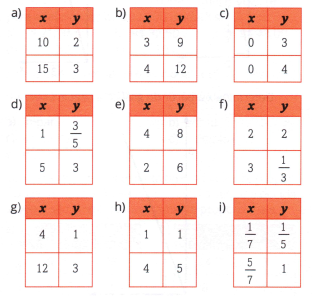
\includegraphics[width=1\linewidth]{8FMA03_imagens/imagem1}
           \item Sejam $x$ e $y$ variáveis diretamente proporcionais. Complete a tabela a seguir:
           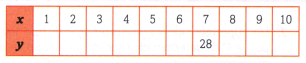
\includegraphics[width=1\linewidth]{8FMA03_imagens/imagem2}
		\end{enumerate}
    \end{multicols}
\end{document}